\section{Системийн шаардлага}

\subsection{Функционал шаардлагууд}
\begin{itemize}
      \item[] /ФШ 10/ Систем нь цахим бүтээл болон лицензийн талаарх мэдээллийн найдвартай байдлыг хадгалахын тулд блокчэйнтэй харилцах ёстой.
      \item[] /ФШ 20/ Системд хэрэглэгчид крипто хэтэвчээ ашиглан өөрийгөө баталгаажуулах боломжтой байх ёстой (жишээ нь, MetaMask).
      \item[] /ФШ 30/ Системд зөвхөн холбогдсон түрийвчтэй, баталгаажуулсан хэрэглэгчид системийн функцэд хандах эрхтэй байх ёстой.
      \item[] /ФШ 40/ Систем нь хэрэглэгчдэд янз бүрийн төрлийн цахим бүтээлийг (жишээ нь, видео, аудио, PDF, зураг) аюулгүйгээр байршуулах боломжтой байх ёстой.
      \item[] /ФШ 50/ Систем нь цахим бүтээлийг байршуулахдаа бүтээлийн мэдээллийг бүртгэх мөн үнийг тогтоох боломжтой байх ёстой.
      \item[] /ФШ 60/ Систем нь өгөгдлийн нууцлал, аюулгүй байдлыг хангах үүднээс байршуулахаас өмнө файлуудыг шифрлэн IPFS (InterPlanetary File System) дээр найдвартай хадгалах ёстой.
      \item[] /ФШ 70/ Систем нь шифрлэгдсэн файлуудыг зохих зөвшөөрөлтэй эрх бүхий хэрэглэгчдэд зориулан тайлах ёстой.
      \item[] /ФШ 80/ Системд хэрэглэгчдэд цахим бүтээлийн үнэд тохирсон шаардлагатай төлбөрийг төлж эзэмшигчдээс тухайн цахим бүтээлд хандах лиценз буюу хандах зөвшөөрөл авах хүсэлт илгээх боломжтой байх ёстой.
      \item[] /ФШ 90/  Системд цахим бүтээл эзэмшигчид лицензийн хүсэлтийг зөвшөөрөх эсвэл татгалзах боломжтой байх ёстой. Зөвшөөрөгдсөн үед худалдан авагчид бүтээлийн лицензийг өгөх мөн зохих төлбөрийг эзэмшигчид шилжүүлэх ёстой.
      \item[] /ФШ 100/  Системд цахим бүтээл эзэмшигчид мөн хэрэглэгчдийн лицензийн хүсэлтээс татгалзах сонголттой байх ёстой. Ийм тохиолдолд төлбөрийг хэрэглэгчдэд буцааж өгөх ёстой.
      \item[] /ФШ 110/  Систем нь цахим бүтээл эзэмших, түүнд лиценз олгох асуудлыг зохицуулахын тулд ухаалаг гэрээг блокчэйн дээр байршуулж, удирдах ёстой.
      \item[] /ФШ 120/  Системд хэрэглэгчид хүссэн үедээ системээс цахим бүтээлийн орлогоо өөрийн крипто хэтэвч рүү татах боломжтой байх ёстой.
      \item[] /ФШ 130/  Систем нь бүтээл байршуулах, удирдах, өмчлөлийг баталгаажуулахын тулд ухаалаг гэрээтэй харилцах ёстой.
      \item[] /ФШ 140/  Хэрэглэгчид cистем дээр байршуулсан цахим бүтээлийн дэлгэрэнгүй мэдээллийг үзэх боломжтой байх ёстой.
      \item[] /ФШ 150/  Цахим бүтээлийн лиценз авахад лицензэд өвөрмөц дугаар олгож, блокчэйн дээр хадгалах ёстой.
      \item[] /ФШ 160/  Систем нь хэрэглэгчид лиценз авсны дараа лицензийн дугаар, файлын мэдээлэл зэрэг лицензийнхээ дэлгэрэнгүй мэдээллийг агуулсан цахим гэрчилгээ олгох ёстой.
\end{itemize}

\subsection{Функционал бус шаардлагууд}
\begin{itemize}
   \item[] /ФБШ 10/ Блокчэйн технологи нь өгөгдлийн бүрэн бүтэн байдлыг хангаж, лицензийн мэдээллийг зөвшөөрөлгүй өөрчлөхөөс сэргийлнэ.
   \item[] /ФБШ 20/ Систем нь гүйцэтгэлийн бууралтгүйгээр олон тооны хэрэглэгчид болон лицензүүдийг зохицуулах чадвартай байх ёстой.
   \item[] /ФБШ 30/ Ухаалаг гэрээ нь модульчлагдсан байх ёстой бөгөөд шинэчлэгдэхэд хялбар байх ёстой.
   \item[] /ФБШ 40/ Систем нь хүлээн зөвшөөрөгдсөн тодорхой хугацааны дотор баталгаажуулах хүсэлтийг хурдан боловсруулах чадвартай байх ёстой.
   \item[] /ФБШ 50/ Систем нь янз бүрийн техникийн чадвартай хэрэглэгчдэд үүнийг үр дүнтэй ашиглах боломжийг олгодог хэрэглэгчдэд ээлтэй интерфейстэй байх ёстой.
   \item[] /ФБШ 50/ Систем нь янз бүрийн үйлдлийн систем, хөтөч, төхөөрөмжтэй нийцтэй байх ёстой.
   \item[] /ФБШ 60/ Систем нь лиценз олгох, дижитал гүйлгээ, блокчэйн технологитой холбоотой аливаа зохицуулалтын шаардлагад нийцэж байх ёстой.
   \item[] /ФБШ 70/ Энэ систем нь гамшгийн үед өгөгдөл алдагдахгүй байхын тулд найдвартай нөөцлөх, сэргээх механизмтай байх ёстой.
\end{itemize}

\newpage
\section{Системийн ажлын явцын диаграмм}
Цахим бүтээлийн ажлын явцыг дараах байдлаар тодорхойлов. Системийн оролцогч талуудыг цахим бүтээлийн лиценз буюу хандах зөвшөөрөл авах гэж буй хэрэглэгч. Нөгөө талаас цахим бүтээл оруулах, түүнд лиценз буюу хандах зөвшөөрөл олгож буй бүтээл эзэмшигч гэж тодорхойлсон.
\begin{figure}[h!]
	\centering
	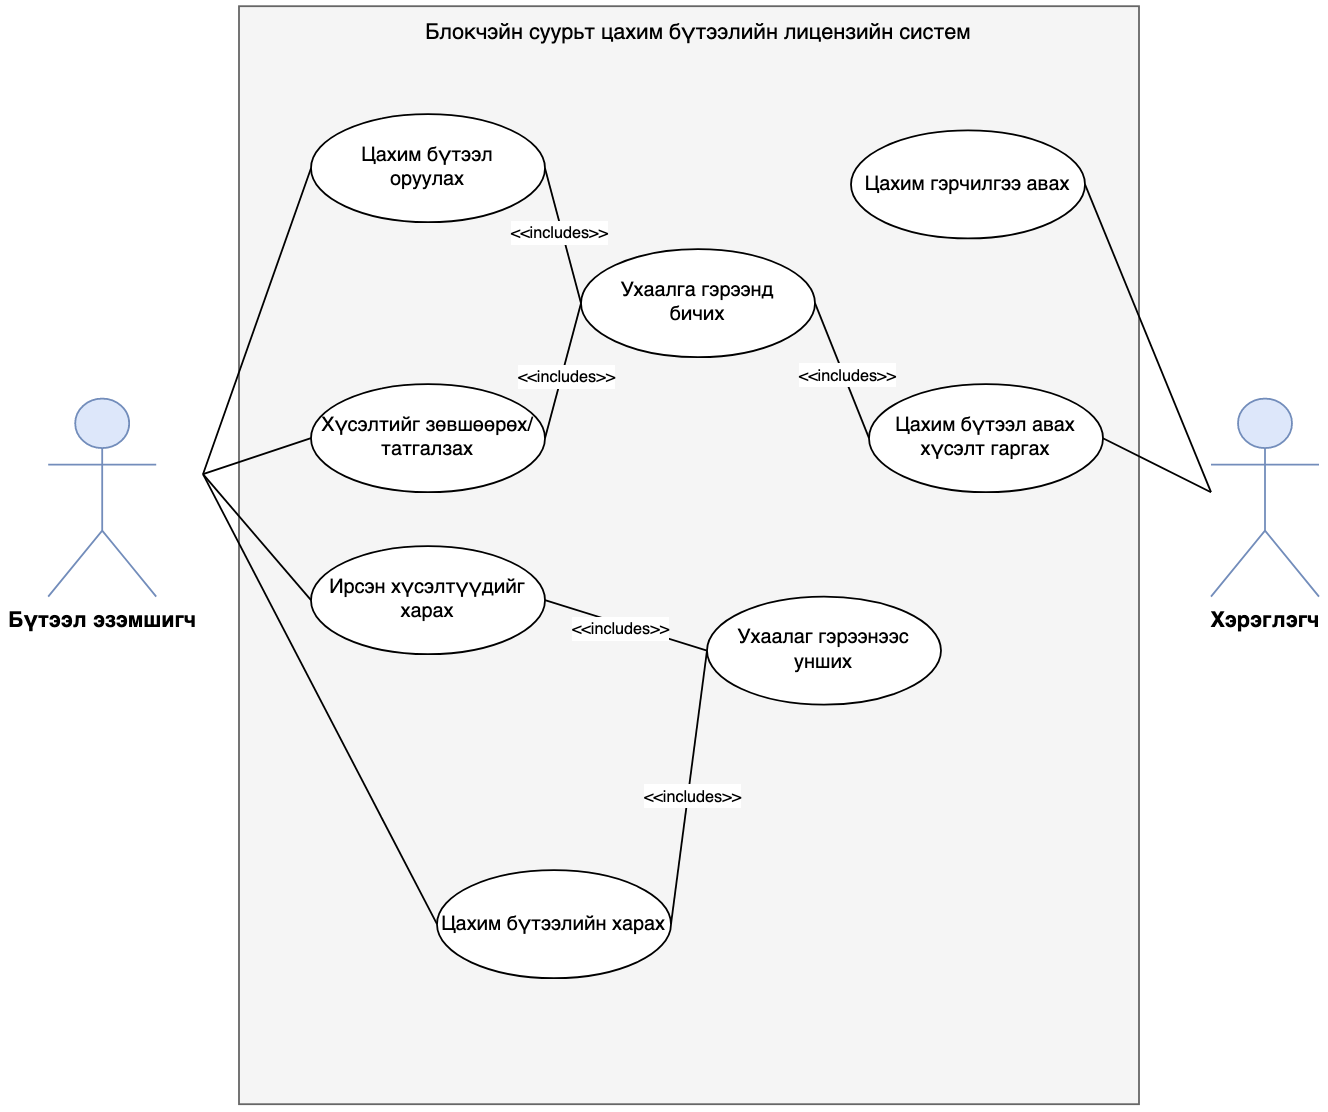
\includegraphics[scale=0.36]{src/images/usecase.png}
	\caption{Use-case диаграмм}
\end{figure}

\pagebreak
\section{Дарааллын диаграмм}
\subsection{Хэрэглэгч цахим бүтээл оруулах дарааллын диаграмм}
\begin{figure}[h!]
	\centering
	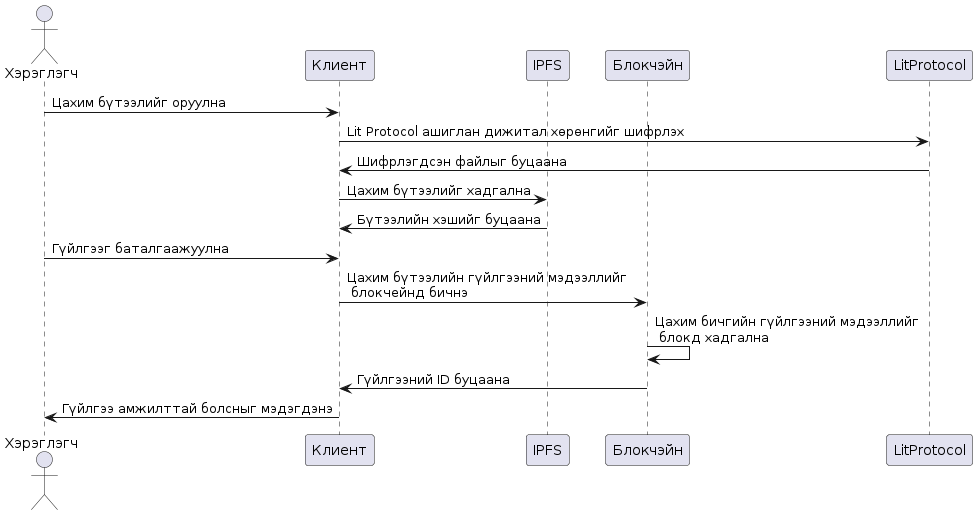
\includegraphics[scale=0.55, angle=90]{src/images/sequence.png}
	\caption{Хэрэглэгч цахим бүтээл оруулах дарааллын диаграмм}
\end{figure}
\subsection{Хэрэглэгч цахим бүтээлд хандах эрх хүсэх дарааллын диаграмм}
\begin{figure}[h!]
	\centering
	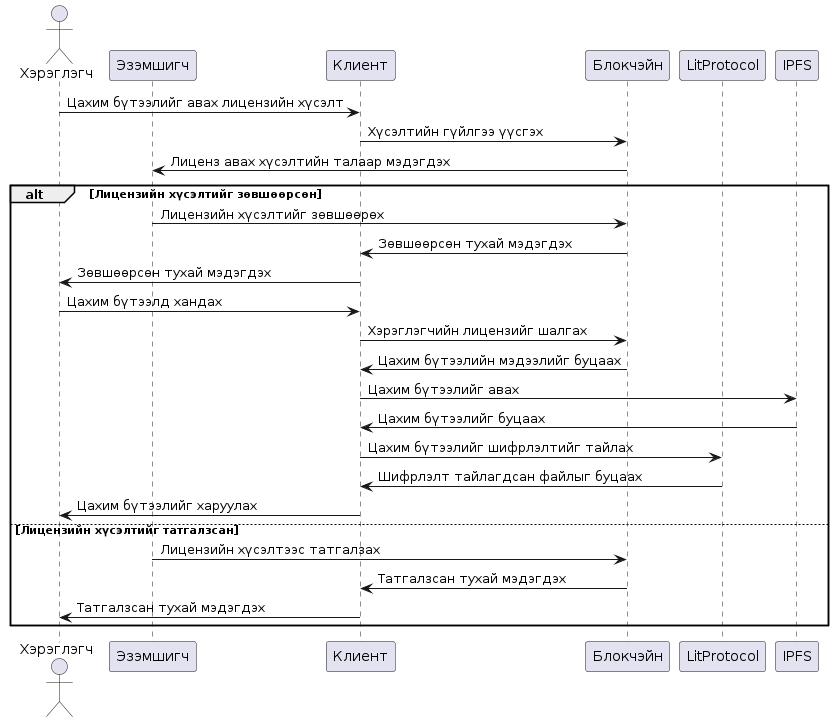
\includegraphics[scale=0.6, angle=90]{src/images/sequence-2.png}
	\caption{Хэрэглэгч цахим бүтээлийг хүсэх дарааллын диаграмм}
\end{figure}

\newpage
\section{Архитектур}
Энэхүү төслийн фронтэнд хэсэг нь NextJS-н ашигласан тул сервер талын рендер хийж байгаа ба хэрэглэгчийн оруулсан цахим бүтээл болон лицензийн мэдээллийг этереум блокчэйн сүлжээнд байршсан ухаалаг гэрээнд бичих болон унших үйлдлийг хийх юм. Мөн хэрэглэгчийн оруулсан цахим бүтээлийн файлыг IPFS сүлжээнд шифрлэн байршуулж, шифрлэлтийн түлхүүрийг Lit сүлжээнд хадгална. Шифрлэлтийн түлхүүрийг хандалтын хяналтын нөхцөлд тодорхойлсны дагуу ухаалаг гэрээгээр зөвшөөрөлтэй эсэхийг шалган авч файлын шифрлэлтийг тайлна.

\begin{figure}[h!]
	\centering
	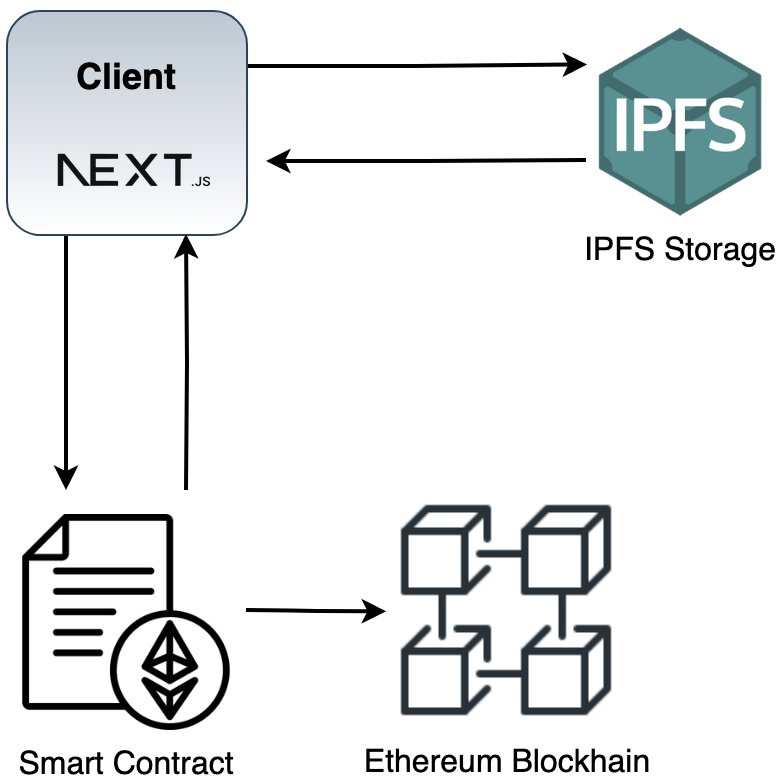
\includegraphics[scale=0.26]{src/images/architecture.png}
	\caption{Системийн ерөнхий архитектур}
\end{figure}
